\documentclass[tikz,border=6pt]{standalone}
\usetikzlibrary{arrows.meta,positioning,calc}
\makeatletter
\AtBeginDocument{\global\let\pgf@selectfontorig\relax}
\makeatother

\tikzset{
  nodebox/.style={draw=black, rounded corners=4pt, very thick, fill=gray!4,
    minimum width=10mm, minimum height=7mm, align=center, inner sep=2pt},
  initial/.style={-Latex, very thick},
  edge/.style={-Latex, thick, shorten >=1pt, shorten <=1pt},
  labelbox/.style={fill=white, inner sep=1.2pt, font=\scriptsize},
  aptxt/.style={font=\scriptsize, text=gray!65!black, anchor=north east},
}

\newcommand{\initarrow}[2]{\draw[initial] #1 -- (#2);}
\newcommand{\statelabel}[2]{\node[aptxt] at ($(#1.south east)+(0.02,-0.05)$) {#2};}

\begin{document}
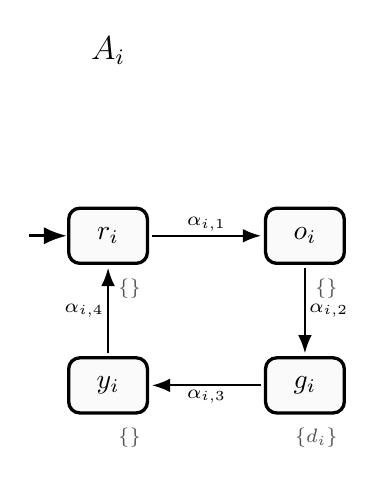
\begin{tikzpicture}[scale=1, transform shape]
  \node[font=\bfseries\large] at (0, 2.35) {$A_i$};

  \node[nodebox] (r) at (0, 0) {$r_i$};
  \node[nodebox] (o) at (2.5, 0) {$o_i$};
  \node[nodebox] (g) at (2.5, -1.9) {$g_i$};
  \node[nodebox] (y) at (0, -1.9) {$y_i$};

  \statelabel{r}{$\{\}$};
  \statelabel{o}{$\{\}$};
  \statelabel{g}{$\{d_i\}$};
  \statelabel{y}{$\{\}$};

  \initarrow{(-1.0, 0)}{r.west}

  \draw[edge] (r) -- node[labelbox, above] {$\alpha_{i,1}$} (o);
  \draw[edge] (o) -- node[labelbox, right] {$\alpha_{i,2}$} (g);
  \draw[edge] (g) -- node[labelbox, below] {$\alpha_{i,3}$} (y);
  \draw[edge] (y) -- node[labelbox, left] {$\alpha_{i,4}$} (r);
\end{tikzpicture}
\end{document}
